\documentclass[10pt,a4paper]{amsart}
\usepackage[margin=19mm]{geometry}
\usepackage{amsmath,amssymb,mathtools}
\usepackage[scr=rsfs,cal=euler]{mathalfa}
\usepackage{xfrac}
\usepackage[unicode,hidelinks,bookmarks=false]{hyperref}
\newcommand{\ie}{i.e.\ }
\newcommand{\cf}{cf.\ }
\newcommand{\resp}{respectively\ }
\newcommand{\Subsection}{\subsection}
\providecommand{\nobreakdash}{\nobreak\hbox{-}}
\setlength{\emergencystretch}{2em}
\multlinegap0pt
\usepackage{tikz}
\usetikzlibrary{cd}
\usepackage{tikz}
\usepackage[shortlabels]{enumitem}
\usepackage{mathtools}
\usepackage{amssymb}
\newtheorem{proposition}{Proposition}
\newtheorem{scope}{Scope}
\usepackage{cleveref}
\crefname{proposition}{Proposition}{Propositions}
\crefname{scope}{Scope}{Scopes}
\newcommand\bft{\mathbf{t}}
\newcommand\bfx{\mathbf{x}}
\newcommand\cG{\mathcal{G}}
\DeclareMathOperator{\lk}{lk}
\DeclareMathOperator{\proj}{Proj}
\newcommand\sfG{\mathsf{G}}
\renewcommand{\tilde}{\widetilde}
\title{Extending Goldberg's Exact Sequence \\ to Braid Groups of Graphs and Simplicial Complexes}
\author{Byung Hee An}
\date{Source: arXiv:2608.14350v1 (CC BY 4.0)}
\begin{document}
\maketitle

\noindent\emph{Source and licence.} Extending Goldberg's Exact Sequence \\ to Braid Groups of Graphs and Simplicial Complexes. Version arXiv:2608.14350v1 (CC BY 4.0), distributed by arXiv under the Creative Commons Attribution 4.0 International licence, http://creativecommons.org/licenses/by/4.0/, as recorded in the arXiv licence metadata for this exact version and shown on the abstract page https://arxiv.org/abs/2608.14350v1. Full licence notice: \texttt{licenses/arxiv-2608.14350-CC-BY-4.0.txt}.\par\smallskip

\noindent\textit{Editorial scope.} Counted unit: the article's proposition prop:valency-decomp (source0.tex lines 2344--2377). The article's complete original proof of it is delivered with it (source0.tex lines 2379--2755, one \texttt{proof} environment of 377 lines). No mathematics is written, repaired or re-derived: the statement and the proof are the article's own lines, in the article's own notation, and no retained line is substituted or re-flowed.  No further source-local context is needed: every cross-reference of every retained line resolves inside the two delivered spans.  Nothing was omitted from any retained span, so the package carries no omission record.  No retained line contains a citation, so the wrapper carries no bibliography and no bibliography entry.  The retained lines contain the article's own diagram code, which the wrapper typesets with the standard tikz packages; no image file is delivered and the package declares no asset dependency.  Editorial formatting only, in addition: an AMS \texttt{amsart} preamble that restates the article's own declarations and macros used by the retained lines, namely the environments \texttt{proposition}, \texttt{scope} on separate counters, together with the standard packages those lines need.  The retained environments print in this document as Proposition 1, Scope 1 in order of appearance, whereas the article prints the same items with the numbering of its own full document.  The complete native source of the article as distributed in the arXiv e-print for this exact version is bundled unchanged as \texttt{sources/207662/source0.tex}.
\begin{proposition}\label{prop:valency-decomp}
The ordered configuration space \(F_n(X)\) is homotopy equivalent to the \emph{graph-of-spaces}
\(\cG_n(X,x)\) over the underlying \emph{distribution graph} \(\sfG_n(X,x)\) described as follows:
\begin{enumerate}[label=(\roman*),leftmargin=2em]
    \item the vertex spaces of \(\cG_n(X,x)\) are the connected
          components of \(F_n(X_x)\), together with the connected
          components of \(n\) copies
          \(\{F_{n-1}^i(X_x):i=1,\dots,n\}\) of \(F_{n-1}(X_x)\);
    \item the edge spaces of \(\cG_n(X,x)\) are the connected
          components of \(F_{n-1}^i(X_x)\times L^j\) for each \(1\le i\le n, 1\le j\le k\); each such edge space
          \(C\times L^j\) (with \(C\in\pi_0(F_{n-1}^i(X_x))\)) is
          attached by the two maps
          \[
            \begin{tikzcd}[column sep=large]
              F_n(X_x) &
              C\times L^j
                \arrow[l, "\phi_{ij}"']
                \arrow[r, "\proj_1"]
              & F_{n-1}^i(X_x),
            \end{tikzcd}
          \]
          where \(\proj_1\) is the projection onto the
          first factor and \(\phi_{ij}\) is induced (up to homotopy)
          by inserting each point of \(L_j\) as the \(i\)-th
          coordinate.
\end{enumerate}
In particular the total numbers of vertices and edges of
\(\cG_n(X,x)\) are
\[
\bigl|\pi_0(F_n(X_x))\bigr|+n\cdot\bigl|\pi_0(F_{n-1}(X_x))\bigr|
\quad\text{ and }\quad
nk\cdot \bigl|\pi_0(F_{n-1}(X_x))\bigr|.
\]
\end{proposition}

\begin{proof}
Define
\[
F_n'(X) \subseteq F_n(X)
\]
to be the subspace consisting of those configurations
\((x_1,\dots,x_n)\in F_n(X)\) with \emph{at most one} coordinate
lying in \(U_x\).

\smallskip
\noindent\emph{Step 1: \(F_n(X)\simeq F_n'(X)\).}
For \(0\le m\le n\) let
\[
F_n(X)^{(m)}\coloneqq
\bigl\{\bfx\in F_n(X) : \#\{i : x_i\in U_x\}\le m\bigr\},
\]
a closed subspace of \(F_n(X)\) -- in a limit, the number of
coordinates lying in the open set \(U_x\) cannot increase -- so
that \(F_n(X)^{(n)}=F_n(X)\) and \(F_n(X)^{(1)}=F_n'(X)\). We
produce a chain of deformation retractions
\[
F_n(X)=F_n(X)^{(n)}\simeq F_n(X)^{(n-1)}\simeq\cdots
\simeq F_n(X)^{(1)}=F_n'(X).
\]

After a further subdivision, the closed star \(\overline{U_x}\)
is collared in \(X\), so there is an open neighbourhood
\(W_x\supseteq\overline{U_x}\) with
\[
W_x\cong\lk_X(x)\times[0,2)\big/\lk_X(x)\times\{0\},
\]
whose radial coordinate extends the cone parametrisation of
\(U_x=\{t<1\}\). Define \(t\colon X\to[0,2]\) by letting
\(t(y)\) be the radial coordinate of \(y\) for \(y\in W_x\) and
\(t(y)\coloneqq2\) otherwise; then \(t\) is continuous, and
\(\bft\coloneqq t\times\cdots\times t\colon X^n\to[0,2]^n\) is
well defined. In a configuration at most one coordinate equals
\(x\), that is, at most one \(t\)-coordinate vanishes; hence
\(\bft(F_n(X))\) misses every face of \([0,2]^n\) through the
origin \(\mathbf0\) of codimension at least \(2\), and lands in
\[
K_n\coloneqq[0,2]^n\setminus
\bigcup_{|I|\le n-2}F_I,
\qquad
F_I\coloneqq\bigl\{\bft : t_j=0\text{ for all }j\notin
I\bigr\}.
\]

Since \(\mathbf0\notin K_n\), the target retracts radially away
from the origin: for \(\bft\neq\mathbf0\) put
\(s\coloneqq\|\bft\|_\infty\in(0,2]\) and
\[
r_n(\bft)\coloneqq\frac{1}{\min\{s,1\}}\bft,
\]
which collapses the portion \(s\in(0,1]\) of each ray issuing
from \(\mathbf0\) onto its endpoint \(s=1\) and leaves the
region \(\{s\ge1\}\) pointwise fixed. Each coordinate hyperplane
\(\{t_i=0\}\) is invariant under scaling, so the excluded faces
are preserved and \(r_n\) restricts to \(K_n\), together with
its straight-line homotopy from the identity.

The retraction lifts to
\(\tilde r_n\colon X^n\setminus\{(x,\dots,x)\}\to
X^n\setminus\{(x,\dots,x)\}\), simply by changing the
\(t\)-coordinates: each coordinate \(x_i\in W_x\) moves radially
outward in its cone fibre until its \(t\)-value becomes
\(\lambda\,t(x_i)\), where \(\lambda=1/\min\{s,1\}\), and the
coordinates outside \(W_x\) stay put (consistently so: if some
coordinate lies outside \(W_x\), then \(s=2\), \(\lambda=1\) and
nothing moves). On each fibre \(\{\theta\}\times[0,2)\) the map
\(t\mapsto\lambda t\) is strictly increasing, so distinct
coordinates remain distinct and \(\tilde r_n\), together with
its straight-line homotopy, restricts to \(F_n(X)\). Along this
homotopy every coordinate moves radially outward, so the number
of coordinates in \(U_x\) never increases and each
\(F_n(X)^{(m)}\) is invariant; at its end
\(\|\bft\|_\infty\ge1\), so not all \(n\) coordinates lie in
\(U_x\) and the image of \(F_n(X)^{(n)}\) is contained in
\(F_n(X)^{(n-1)}\). Moreover a configuration of
\(F_n(X)^{(n-1)}\) has some coordinate outside \(U_x\), hence
\(s\ge1\), \(\lambda=1\), and is fixed pointwise throughout the
homotopy: \(\tilde r_n\) is a deformation retraction of
\(F_n(X)^{(n)}\) onto \(F_n(X)^{(n-1)}\).

Now iterate on the faces through the origin of successive
dimensions. Write
\(K_{n-1}\coloneqq r_n(K_n)=\{\bft\in K_n:\|\bft\|_\infty\ge1\}\),
and fix \(1\le \ell\le n-2\). For a subset
\(I\subseteq\{1,\dots,n\}\) with \(|I|=\ell\), the face \(F_I\)
is excluded from \(K_n\), and the transverse radial parameter
\(s_I\coloneqq\max_{j\notin I}t_j\) is positive throughout
\(K_n\) -- its vanishing would put \(n-\ell\ge2\) coordinates at
\(0\). Let \(\rho_I\) rescale the coordinates \(t_j\),
\(j\notin I\), by \(1/\min\{s_I,1\}\), keeping \(t_i\), \(i\in
I\), fixed: this is the radial retraction away from \(F_I\),
again collapsing the transverse rays onto the fixed region
\(\{s_I\ge1\}\), and \(r_{n-\ell}\) is defined
as the composition of the \(\rho_I\) over all \(I\) with
\(|I|=\ell\), in any fixed order (say lexicographic). As before,
\(r_{n-\ell}\) preserves the excluded faces and lifts to a
self-homotopy \(\tilde r_{n-\ell}\) of the identity of
\(F_n(X)^{(n-\ell)}\), moving the coordinates \(x_j\),
\(j\notin I\), radially outward, one factor \(\rho_I\) after the
other. No stage ever decreases a \(t\)-value, so each
\(F_n(X)^{(m)}\) is invariant and the exit property of each
factor -- \emph{some \(t_j\ge1\) with \(j\notin I\)} -- persists
through the later factors. At the end this property holds for
\emph{every} \(I\) of size \(\ell\). Consequently no
configuration in the image has \(n-\ell\) or more coordinates in
\(U_x\): the set \(I_0\) of indices \emph{outside} \(U_x\) would
have \(|I_0|\le\ell\), and enlarging it to any \(I\supseteq I_0\)
with \(|I|=\ell\) would leave \(t_j<1\) for all \(j\notin I\), a
contradiction. Hence the image of \(F_n(X)^{(n-\ell)}\) lies in
\(F_n(X)^{(n-\ell-1)}\). Moreover a configuration of
\(F_n(X)^{(n-\ell-1)}\) has at least \(\ell+1\) coordinates
outside \(U_x\), so for every \(I\) with \(|I|=\ell\) some
\(j\notin I\) has \(t_j\ge1\), every factor \(\rho_I\) acts as
the identity on it, and it is fixed pointwise: as before,
\(\tilde r_{n-\ell}\) is a deformation retraction of
\(F_n(X)^{(n-\ell)}\) onto \(F_n(X)^{(n-\ell-1)}\).

Running \(\ell=1,\dots,n-2\) completes the chain and yields
\(F_n(X)\simeq F_n'(X)\). (In the target, the final image
\(K_1\) meets the unit cube \([0,1]^n\) in the \(1\)-dimensional
union of the segments with at least \(n-1\) coordinates equal to
\(1\), matching the fact that at most one configuration point
survives inside \(U_x\).) \cref{fig:K1-cube} illustrates the
case \(n=3\).

\begin{figure}[ht]
\centering
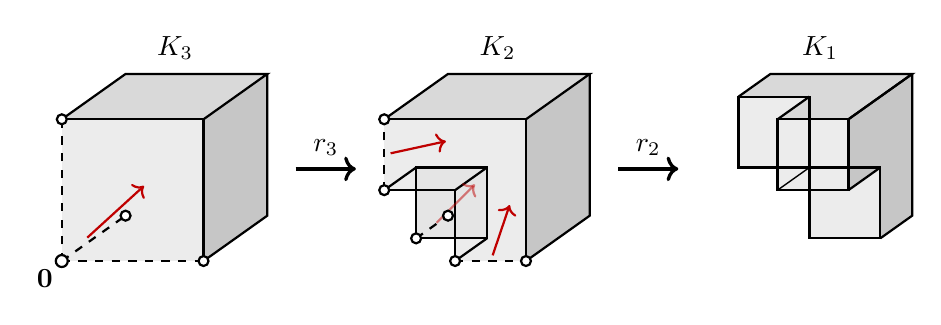
\begin{tikzpicture}[line width=0.8pt, scale=0.9]

\begin{scope}
  \fill[gray!15] (0,0) -- (2,0) -- (2,2) -- (0,2) -- cycle;
  \fill[gray!30] (0,2) -- (2,2) -- (2.9,2.64) -- (0.9,2.64) -- cycle;
  \fill[gray!45] (2,0) -- (2,2) -- (2.9,2.64) -- (2.9,0.64) -- cycle;
  \draw[dashed] (0,0) -- (2,0);
  \draw[dashed] (0,0) -- (0,2);
  \draw[dashed] (0,0) -- (0.9,0.64);
  \draw (2,0) -- (2,2) -- (0,2);
  \draw (0,2) -- (0.9,2.64) -- (2.9,2.64) -- (2,2);
  \draw (2,0) -- (2.9,0.64) -- (2.9,2.64);
  \draw[->, red!75!black, thick] (0.36,0.33) -- (1.16,1.06);
  \filldraw[fill=white] (0,0) circle (2.4pt);
  \filldraw[fill=white] (2,0) circle (2.0pt);
  \filldraw[fill=white] (0,2) circle (2.0pt);
  \filldraw[fill=white] (0.9,0.64) circle (2.0pt);
  \node[below left=-1pt] at (-0.02,-0.02) {\(\mathbf0\)};
  \node at (1.6,3.0) {\(K_3\)};
\end{scope}

\draw[->, very thick] (3.3,1.3) -- (4.15,1.3)
  node[midway, above=1pt] {\(r_3\)};

\begin{scope}[xshift=4.55cm]
  \fill[gray!15] (1,0) -- (2,0) -- (2,2) -- (0,2) -- (0,1) -- (1,1) -- cycle;
  \fill[gray!20] (0.45,0.32) -- (1.45,0.32) -- (1.45,1.32) -- (0.45,1.32) -- cycle;
  \fill[gray!30] (0,2) -- (2,2) -- (2.9,2.64) -- (0.9,2.64) -- cycle;
  \fill[gray!45] (2,0) -- (2,2) -- (2.9,2.64) -- (2.9,0.64) -- cycle;
  \draw (0.45,0.32) -- (1.45,0.32) -- (1.45,1.32) -- (0.45,1.32) -- cycle;
  \draw (1,0) -- (1.45,0.32);
  \draw (1,1) -- (1.45,1.32);
  \draw (0,1) -- (0.45,1.32);
  \draw (1,0) -- (1,1) -- (0,1);
  \draw[dashed] (1,0) -- (2,0);
  \draw[dashed] (0,1) -- (0,2);
  \draw[dashed] (0.45,0.32) -- (0.9,0.64);
  \draw (2,0) -- (2,2) -- (0,2);
  \draw (0,2) -- (0.9,2.64) -- (2.9,2.64) -- (2,2);
  \draw (2,0) -- (2.9,0.64) -- (2.9,2.64);
  \draw[->, red!75!black, thick] (1.53,0.08) -- (1.77,0.79);
  \draw[->, red!75!black, thick] (0.09,1.52) -- (0.87,1.69);
  \draw[->, red!75!black, thick, opacity=0.5] (0.74,0.54) -- (1.28,1.08);
  \filldraw[fill=white] (1,0) circle (2.0pt);
  \filldraw[fill=white] (2,0) circle (2.0pt);
  \filldraw[fill=white] (0,1) circle (2.0pt);
  \filldraw[fill=white] (0,2) circle (2.0pt);
  \filldraw[fill=white] (0.45,0.32) circle (2.0pt);
  \filldraw[fill=white] (0.9,0.64) circle (2.0pt);
  \node at (1.6,3.0) {\(K_2\)};
\end{scope}

\draw[->, very thick] (7.85,1.3) -- (8.7,1.3)
  node[midway, above=1pt] {\(r_2\)};

\begin{scope}[xshift=9.1cm]
  \fill[gray!15] (1,1) -- (2,1) -- (2,2) -- (1,2) -- cycle;
  \fill[gray!15] (0.45,1.32) -- (1.45,1.32) -- (1.45,2.32) -- (0.45,2.32) -- cycle;
  \fill[gray!15] (1.45,0.32) -- (2.45,0.32) -- (2.45,1.32) -- (1.45,1.32) -- cycle;
  \fill[gray!30] (0.45,2.32) -- (0.9,2.64) -- (2.9,2.64) -- (2,2) -- (1,2) -- (1.45,2.32) -- cycle;
  \fill[gray!45] (2,1) -- (2,2) -- (2.9,2.64) -- (2.9,0.64) -- (2.45,0.32) -- (2.45,1.32) -- cycle;
  \draw (1,1) -- (2,1) -- (2,2) -- (1,2) -- cycle;
  \draw (0.45,1.32) -- (1.45,1.32) -- (1.45,2.32) -- (0.45,2.32) -- cycle;
  \draw (1.45,0.32) -- (2.45,0.32) -- (2.45,1.32) -- (1.45,1.32) -- cycle;
  \draw (0.45,2.32) -- (0.9,2.64) -- (2.9,2.64) -- (2,2);
  \draw (1,2) -- (1.45,2.32);
  \draw (2,2) -- (2.9,2.64);
  \draw (2.9,2.64) -- (2.9,0.64) -- (2.45,0.32);
  \draw (2.45,1.32) -- (2,1);
  \draw[line width=0.5pt] (1,1) -- (1.45,1.32);
  \node at (1.6,3.0) {\(K_1\)};
\end{scope}

\end{tikzpicture}
\caption{Step~1 in the case \(n=3\). In \(K_3\), the origin
\(\mathbf0\) and the three coordinate edges through it are
removed (open circles and dashed lines). The radial deformation
\(r_3\) away from \(\mathbf0\) deletes the corner unit cube,
producing \(K_2\); the transverse deformations \(r_2\) away
from the three removed edges delete three further unit cubes,
leaving \(K_1\), a union of four unit cubes.}
\label{fig:K1-cube}
\end{figure}

\smallskip
\noindent\emph{Step 2: decomposition of \(F_n'(X)\).}
For each \(i\in\{1,\dots,n\}\) define the \(i\)-th
\emph{thickened insertion map}
\[
g_i\colon F_{n-1}\bigl(X\setminus U_x\bigr)
\times U_x \longrightarrow F_n'(X)
\]
by
\[
g_i\bigl((x_1,\dots,\hat{x}_i,\dots,x_n),\,y\bigr)
=
(x_1,\dots,x_{i-1},\,y,\,x_{i+1},\dots,x_n);
\]
this is analogous to \(f_i\) but allows the inserted point \(y\) to
range over the entire neighbourhood \(U_x\). Each \(g_i\) is an open
map, and the images \(g_i(F_{n-1}(X\setminus U_x)\times U_x)\) are
pairwise disjoint as \(i\) varies.

Set
\[
F_n'(X\setminus \overline{V_x})
=
F_n(X\setminus \overline{V_x})\cap F_n'(X)
\subseteq F_n(X),
\]
an open subset of \(F_n'(X)\). It admits the disjoint decomposition
\begin{align*}
F_n'(X\setminus \overline{V_x})
&=
F_n(X\setminus U_x)
\coprod
\left(\coprod_{i=1}^n g_i\bigl(F_{n-1}(X\setminus U_x)
\times (U_x\setminus \overline{V_x})\bigr)\right) \\
&=
F_n(X\setminus U_x)
\coprod
\left(\coprod_{i=1}^n\coprod_{j=1}^k
g_i\bigl(F_{n-1}(X\setminus U_x)\times L^j\times(1/2,1)\bigr)\right).
\end{align*}

On the other hand, \(F_n'(X)\) itself decomposes as a union of
open subsets
\[
F_n'(X)
=
F_n'\bigl(X\setminus \overline{V_x}\bigr)
\cup
\bigcup_{i=1}^n
g_i\bigl(F_{n-1}(X\setminus U_x)\times U_x\bigr),
\]
where the first piece collects the configurations with no
coordinate in \(\overline{V_x}\), and the \(i\)-th \(g_i\)-piece those
whose \(i\)-th coordinate lies in \(U_x\) and whose other coordinates
lie outside \(U_x\). The intersection of the main piece with the
\(i\)-th \(g_i\)-piece is
\begin{align*}
F_n'(X\setminus \overline{V_x})
\cap
g_i\bigl(F_{n-1}(X\setminus U_x)\times U_x\bigr)
&=
g_i\bigl(F_{n-1}(X\setminus U_x)\times (U_x\setminus \overline{V_x})\bigr)\\
&=
\coprod_{j=1}^k g_i\bigl(F_{n-1}(X\setminus U_x)\times L^j\times(1/2,1)\bigr).
\end{align*}

\smallskip
\noindent\emph{Step 3: identifying the pieces up to homotopy.}
It follows directly
that for each \(*=n-1, n\),
\[
F_*'\bigl(X\setminus \overline{V_x}\bigr)
\simeq
F_*\bigl(X\setminus U_x\bigr)
\simeq
F_*(X_x),
\]
and so 
each \(g_i\)-piece \(g_i\bigl(F_{n-1}(X\setminus U_x)\times U_x\bigr)\) is homotopy
equivalent to the image \(f_i(F_{n-1}(X_x))\) of the insertion map
\(f_i\) defined above, and hence to \(F_{n-1}(X_x)\) itself. 
To track the dependence on \(i\), let us
write \(F_{n-1}^i(X_x)\) for the copy of \(F_{n-1}(X_x)\) associated
with the subspace \(f_i(F_{n-1}(X_x))\subseteq F_n(X)\). We then have
\[
g_i\bigl(F_{n-1}(X\setminus U_x)\times U_x\bigr)
\simeq
f_i\bigl(F_{n-1}(X_x)\bigr)
\simeq
F_{n-1}^i(X_x).
\]

Finally, for each \(j\in\{1,\dots,k\}\), we likewise have
\[
g_i\bigl(F_{n-1}(X\setminus U_x)\times L^j\times(1/2,1)\bigr)
\simeq
f_i\bigl(F_{n-1}(X_x)\bigr)\times L^j
\simeq
F_{n-1}^i(X_x)\times L^j.
\]

\smallskip
\noindent\emph{Step 4: assembling the graph-of-spaces.}
We first describe the underlying distribution graph
\(\sfG=\sfG_n(X,x)\). Its vertex set is
\[
V(\sfG) = \pi_0\bigl(F_n(X_x)\bigr)\sqcup
\coprod_{i=1}^{n}\pi_0\bigl(F^i_{n-1}(X_x)\bigr),
\]
with one vertex of \emph{\(F_n\)-type} for each connected
component of \(F_n(X_x)\), and one vertex of
\emph{\(F_{n-1}\)-type}, written \((i,C)\), for each strand
index \(i\) and each component
\(C\in\pi_0\bigl(F^i_{n-1}(X_x)\bigr)\). Its edge set is
\[
E(\sfG) = \bigl\{(i,C,j) :
1\le i\le n,\ C\in\pi_0\bigl(F^i_{n-1}(X_x)\bigr),\
1\le j\le k\bigr\},
\]
with one edge for each connected component \(C\times L^j\) of
the spaces \(F^i_{n-1}(X_x)\times L^j\) -- each link component
\(L^j\) being connected. The edge \((i,C,j)\) joins the
\(F_{n-1}\)-type vertex \((i,C)\) to the \(F_n\)-type vertex
determined by the component of \(F_n(X_x)\) containing the
configurations obtained from those of \(C\) by inserting a
point of \(L_j\times\{3/4\}\) as the \(i\)-th coordinate.

Combining Steps 2 and 3, we see that for each
\((i,j)\in\{1,\dots,n\}\times\{1,\dots,k\}\) there are two natural
maps
\[
\begin{tikzcd}
F_n(X_x) &
F_{n-1}^i(X_x)\times L^j
  \arrow[l, "\phi_{ij}"']
  \arrow[r, "\proj_1"]
& F_{n-1}^i(X_x),
\end{tikzcd}
\]
where \(\proj_1\) is the projection onto the first
factor and \(\phi_{ij}\) is (up to homotopy) the composition
\[
\phi_{ij} \simeq
\Bigl(
F_{n-1}^i(X_x)\times L^j
\xrightarrow{\cong}
F_{n-1}\bigl(X\setminus \overline{U_x}\bigr)\times \bigl(L_j\times\{3/4\}\bigr)
\xrightarrow{g_i}
F_n(X_x)
\Bigr).
\]
The two pieces of Step 2 together with these gluing maps exhibit
\(F_n(X)\) as a graph of spaces with the vertex spaces and edge
spaces described in the proposition.


The total numbers of vertices and edges are therefore
\[
\bigl|\pi_0(F_n(X_x))\bigr|+n\cdot \bigl|\pi_0(F_{n-1}(X_x))\bigr|\quad\text{and}\quad
n\,k \cdot \bigl|\pi_0(F_{n-1}(X_x))\bigr|.\qedhere
\]
\end{proof}

\end{document}
